\section{Formal Analysis Using Alloy}
%%
% Alloy language definition for using with the listings package.
%
% 2017, Daniel Andrade
% BSD 3-Clause License
%%
\definecolor{codegreen}{rgb}{0,0.6,0}
\definecolor{codeblue}{rgb}{0,0.0,0.6}
\lstdefinelanguage{alloy}{
	morekeywords={
		module, open, as,
		private, abstract, sig, extends, in,
		lone, some, one, disj,
		fact, pred, fun, assert,
		run, check,
		for, but, exactly,
		this, not, implies, else, let,
		not, no, set, all, sum,
		iff, or, Int, and,
		none, univ, iden
	},
	sensitive=true,
	morecomment=[l]{//},
	morecomment=[l]{--},
	morecomment=[s]{/*}{*/},
	morestring=[b]{"},
	commentstyle=\color{codegreen},
	keywordstyle=\bf \color{codeblue},
	%literate={->}{$\rightarrow$}1
	% replacing characters can cause problems when copying from PDF to editor
}[keywords,comments,strings]

\lstdefinestyle{alloy}{
	commentstyle=\itshape,
	keywordstyle=\bfseries,
	stringstyle=\itshape,
}

% define command for inline use; usage: \alloy|sig A {f: some B}|
\def\alloy{\lstinline[
	language=alloy,
	style=alloy,
	basicstyle=\ttfamily\small
]}

\renewcommand{\ttdefault}{pcr}  % font type with bfseries and ttfamily
% general definitions
\lstset{
	basicstyle=\ttfamily\large
}

\subsection{Alloy Code}
\lstinputlisting[language=alloy,breaklines=true]{codes/alloy_DREAM.als}
\clearpage

\subsection{Meta Model}

\begin{figure}[H]
  \centering
  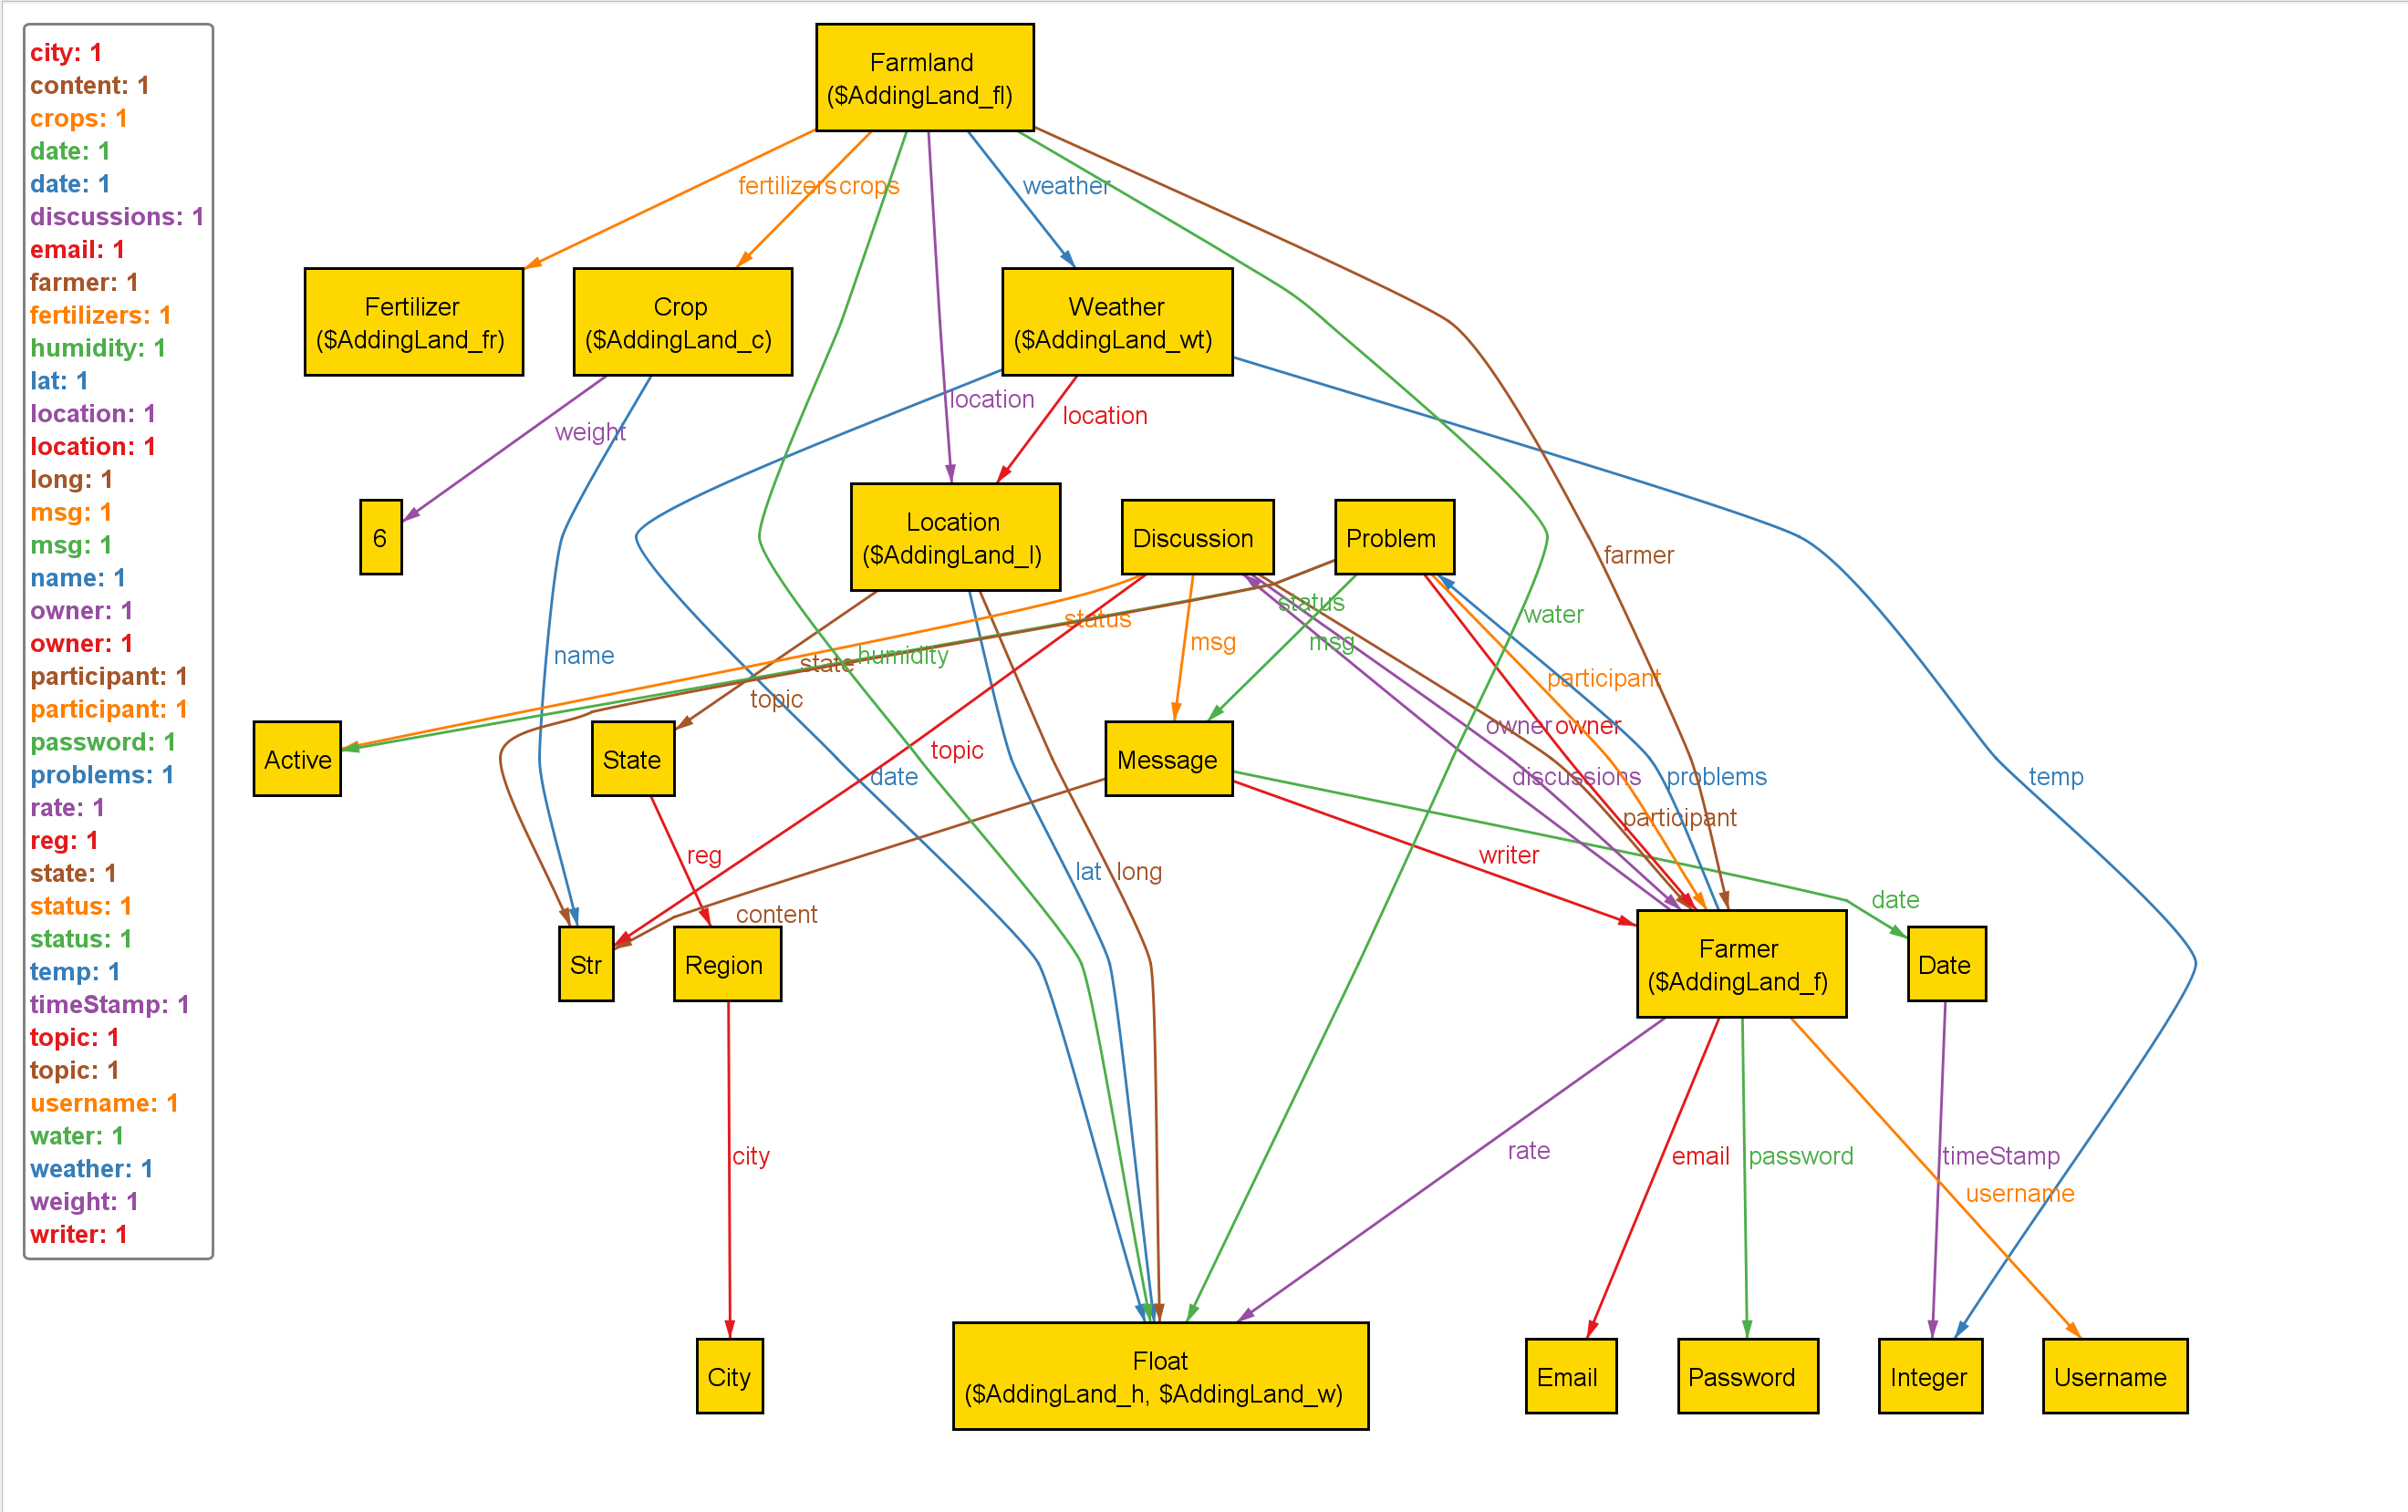
\includegraphics[width=0.9\textheight,keepaspectratio, angle=90]{figures/CreateFarmland1.png}
  \caption{Insert Land}
\end{figure}
\begin{figure}[H]
  \centering
  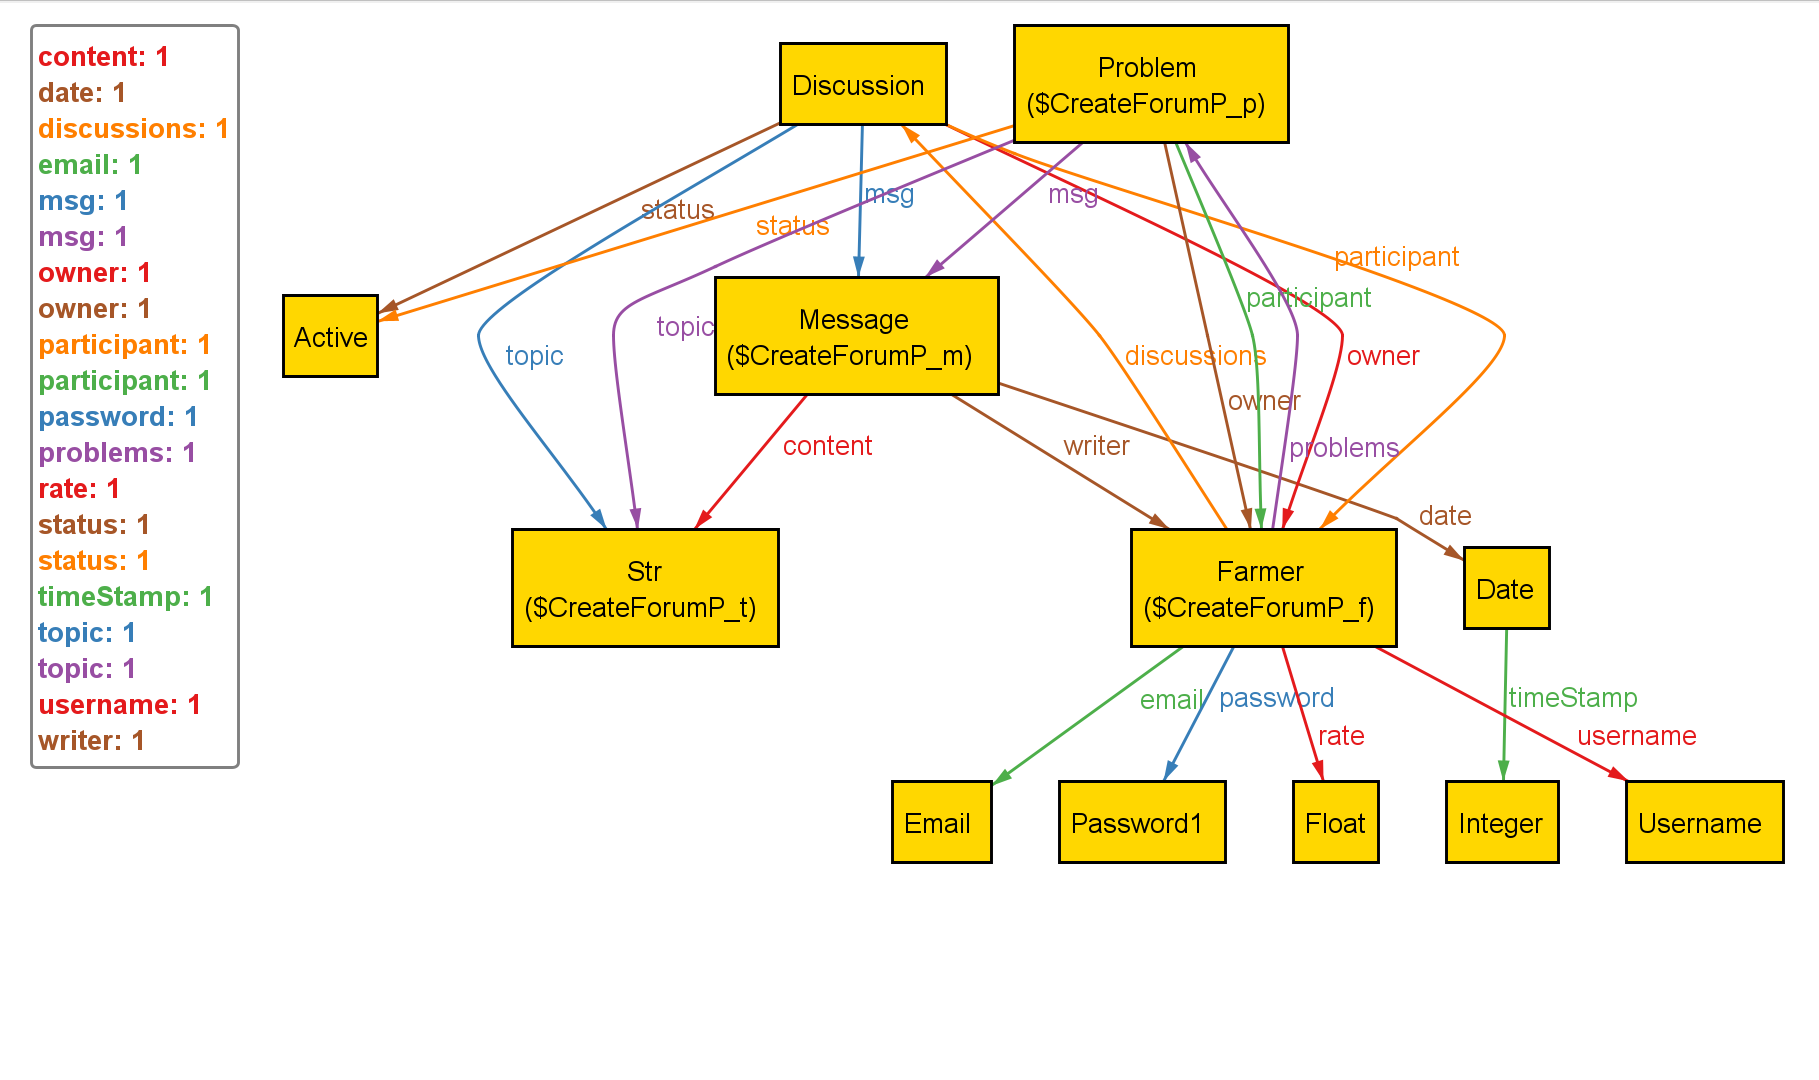
\includegraphics[width=0.9\textheight,keepaspectratio, angle=90]{figures/CreateProblem.png}
  \caption{Create Problem}
\end{figure}
\begin{figure}[H]
  \centering
  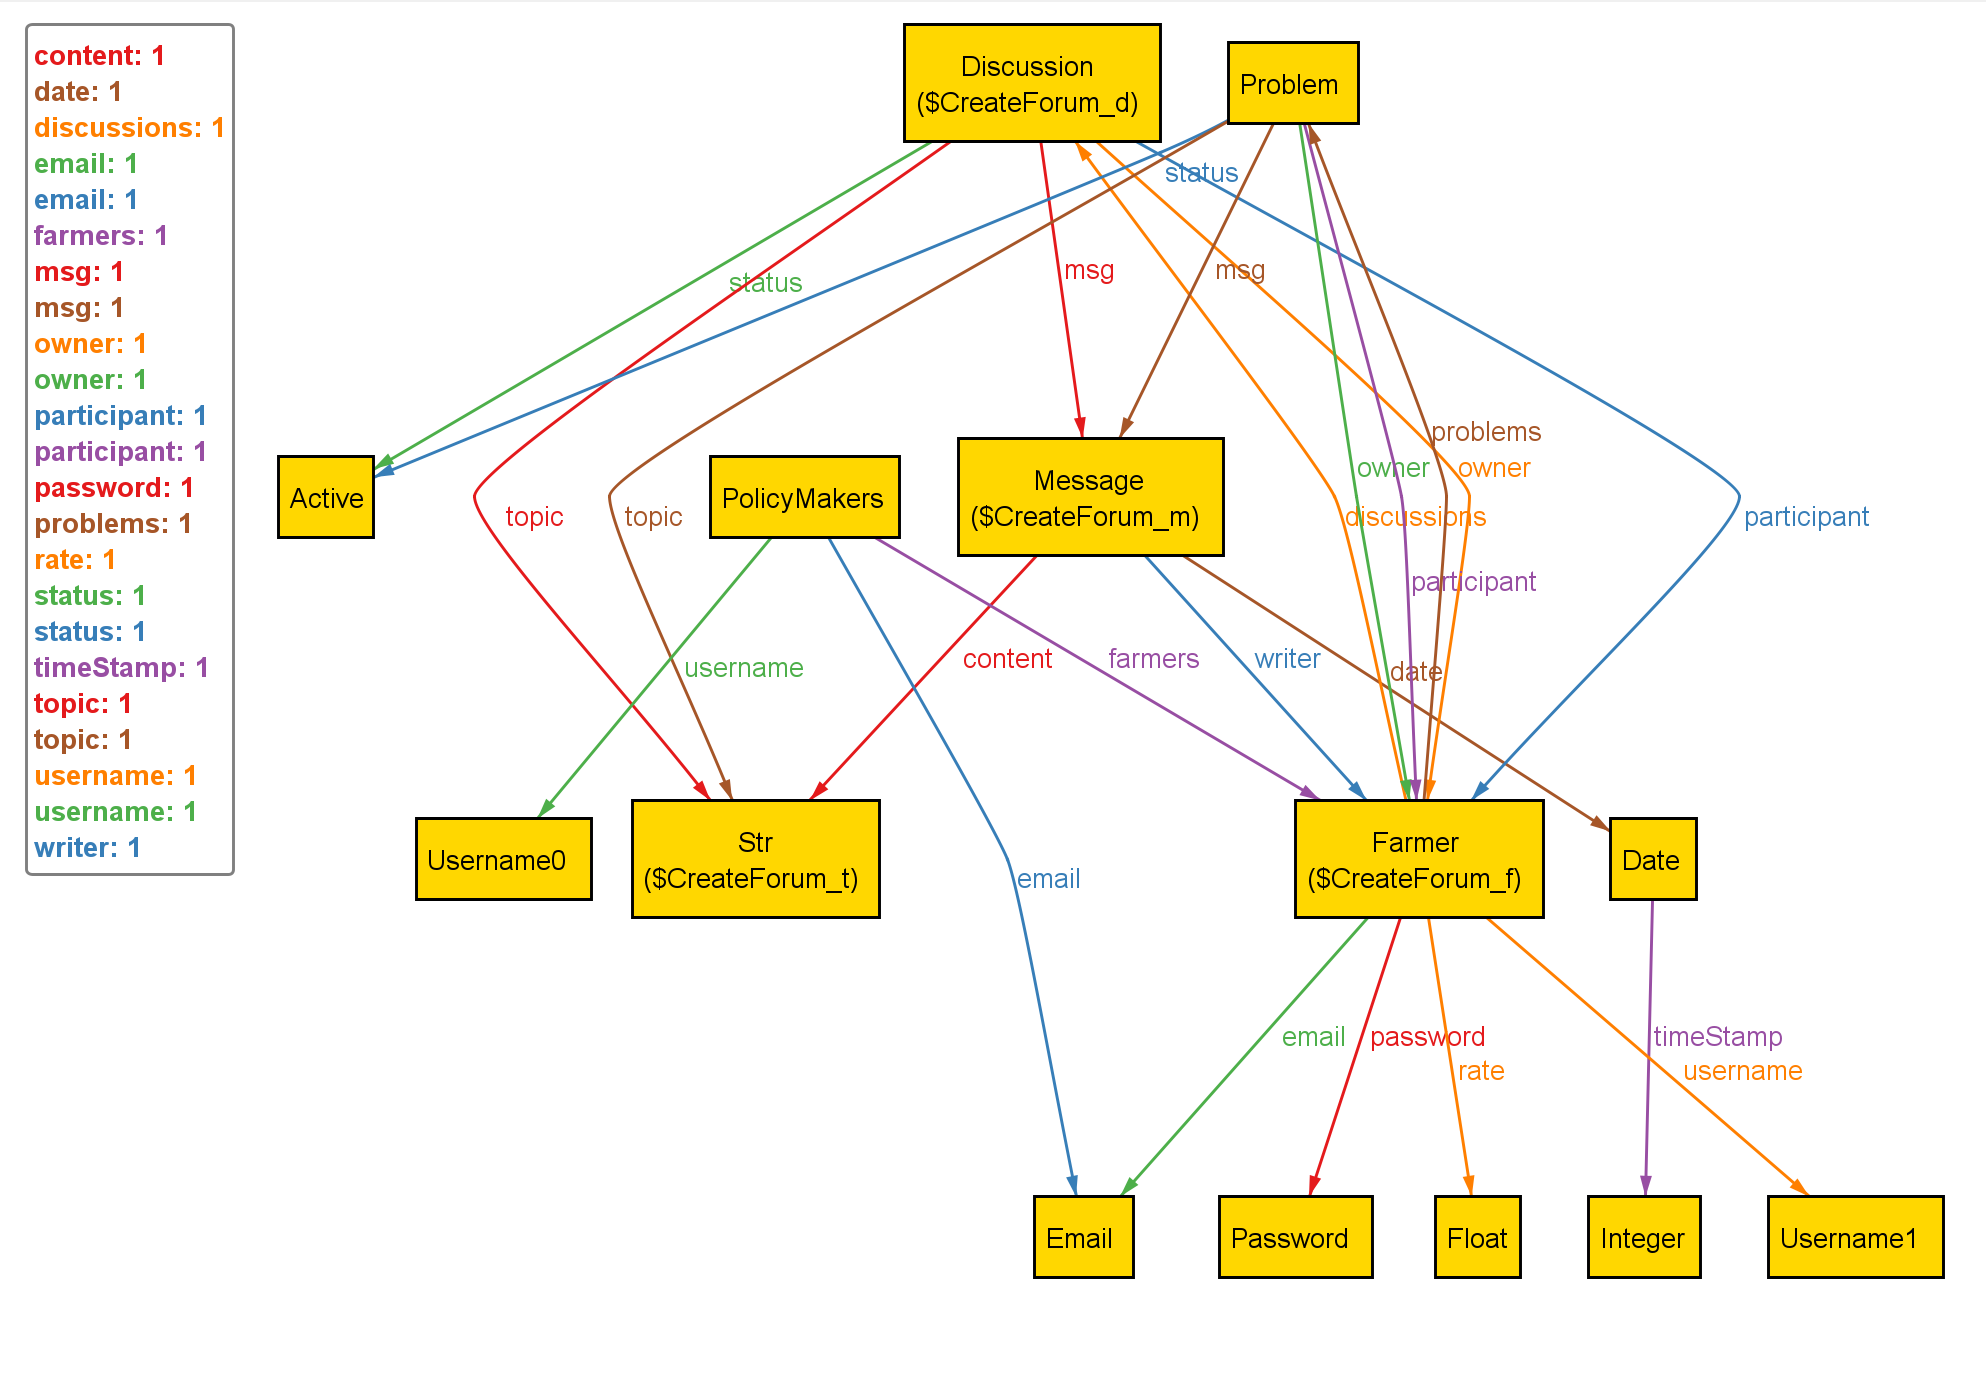
\includegraphics[width=0.9\textheight,keepaspectratio, angle=90]{figures/CreateDiscussion.png}
  \caption{Create Discussion}
\end{figure}
\begin{figure}[H]
  \centering
  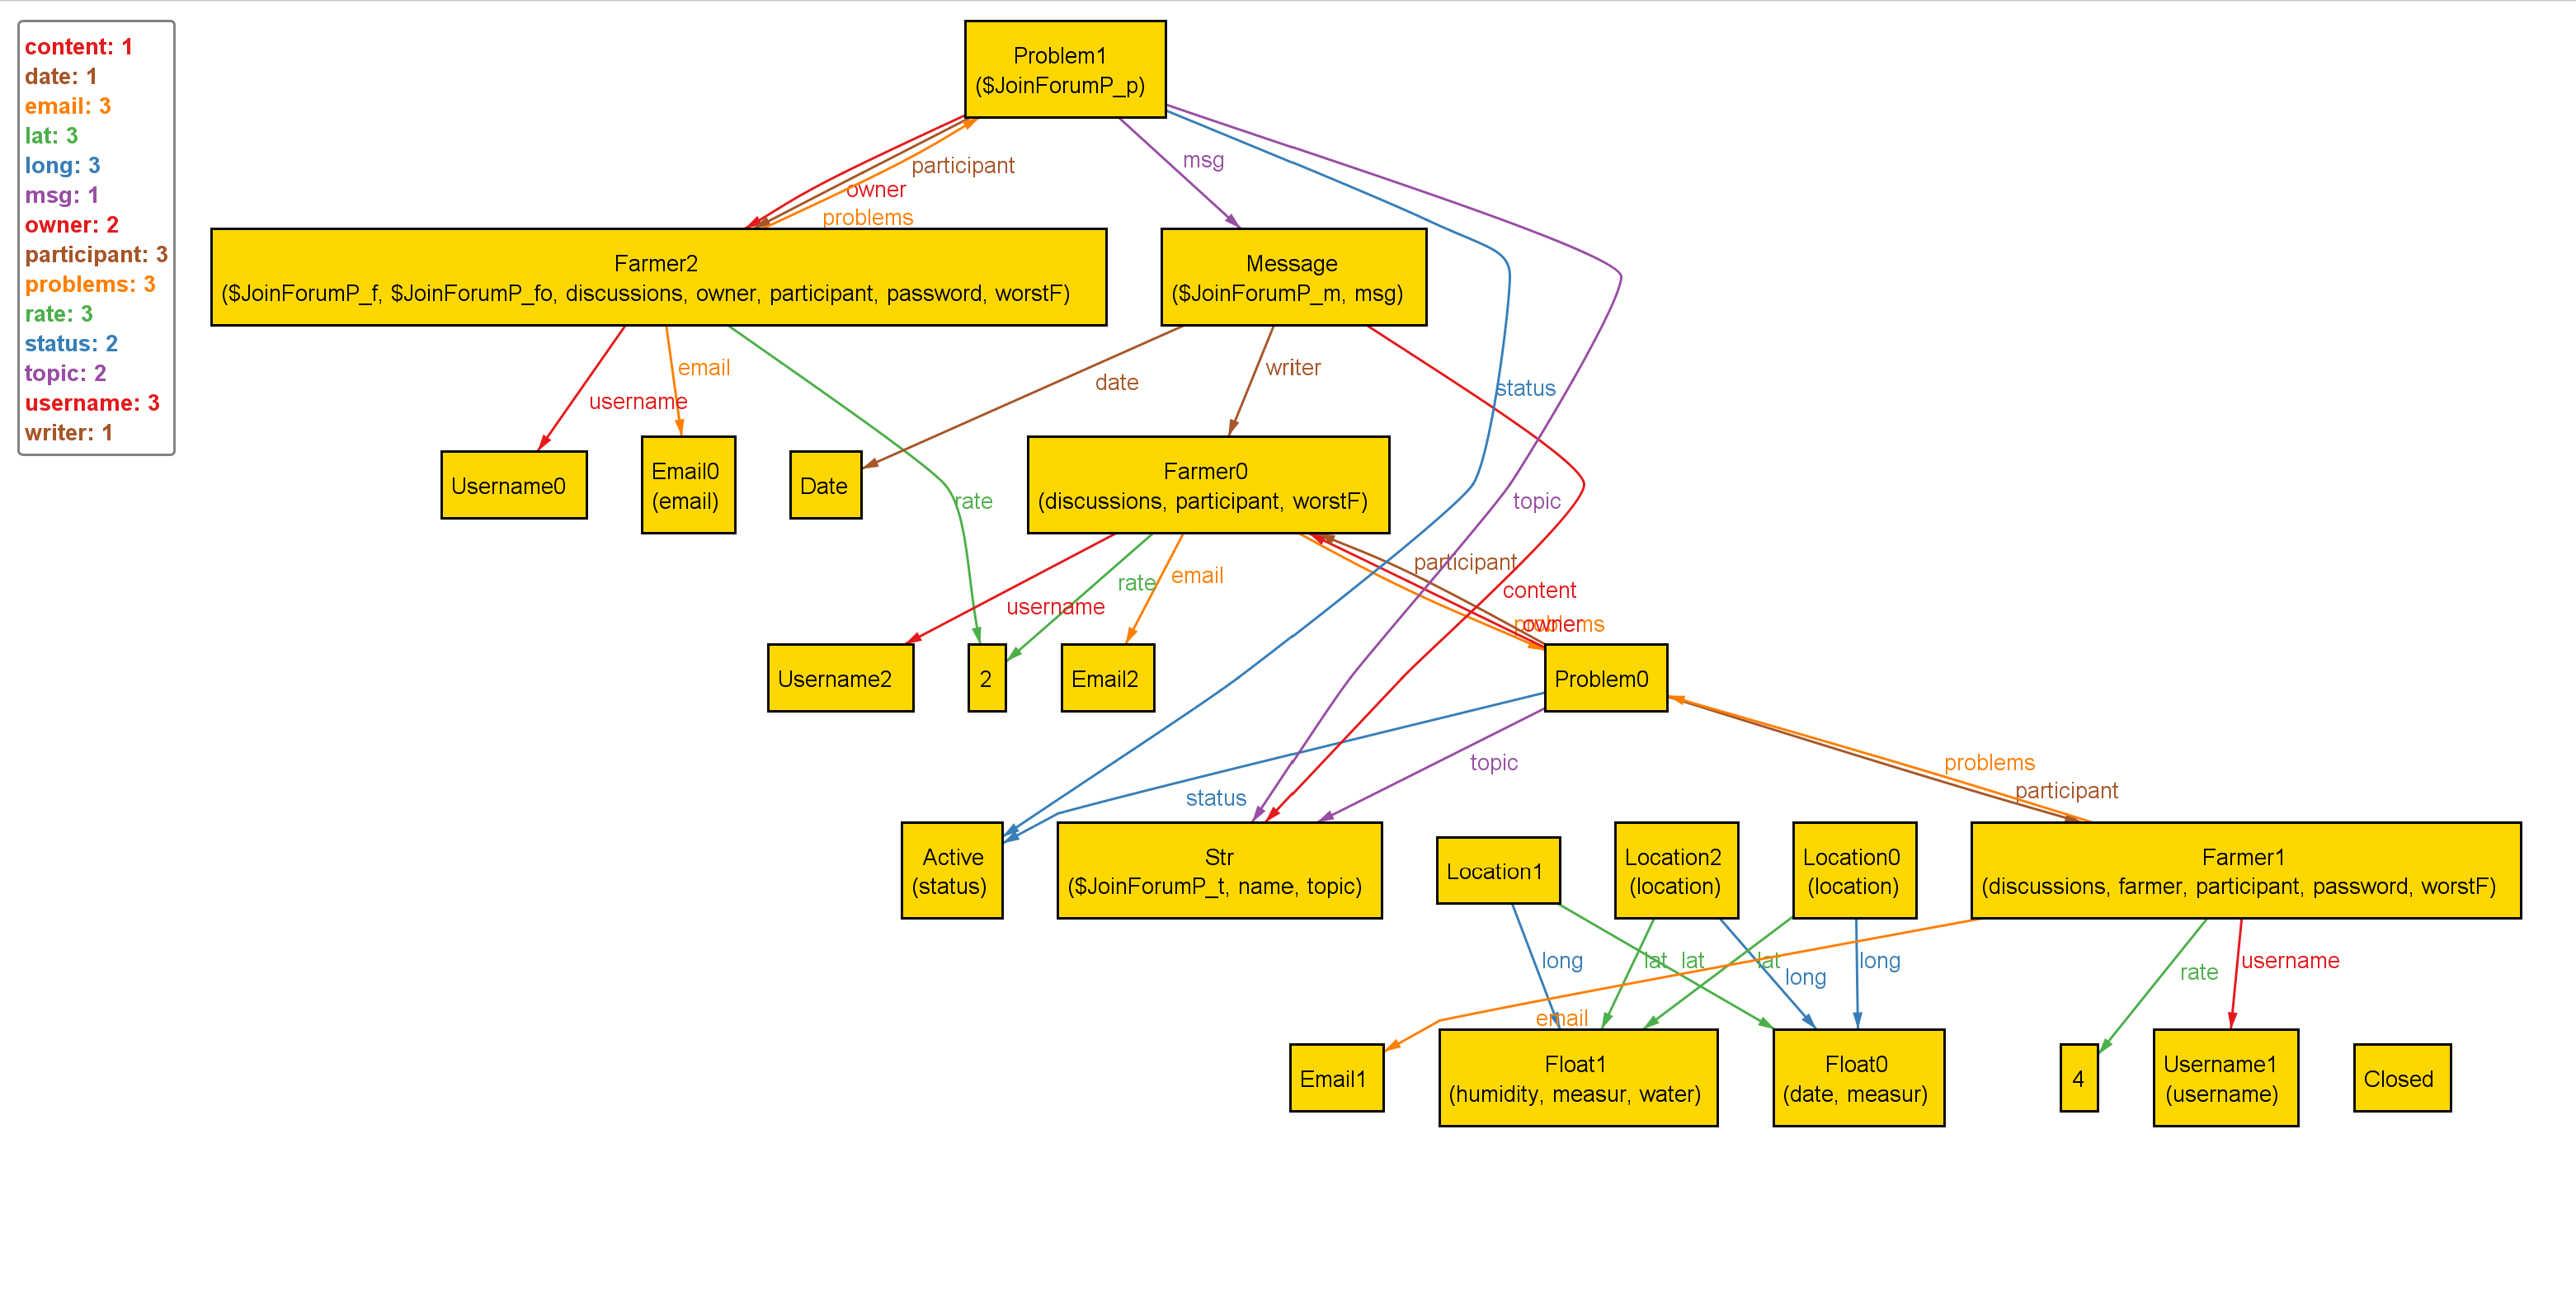
\includegraphics[width=0.9\textheight,keepaspectratio, angle=90]{figures/joinForum.png}
  \caption{Join Forum}
\end{figure}
\begin{figure}[H]
  \centering
  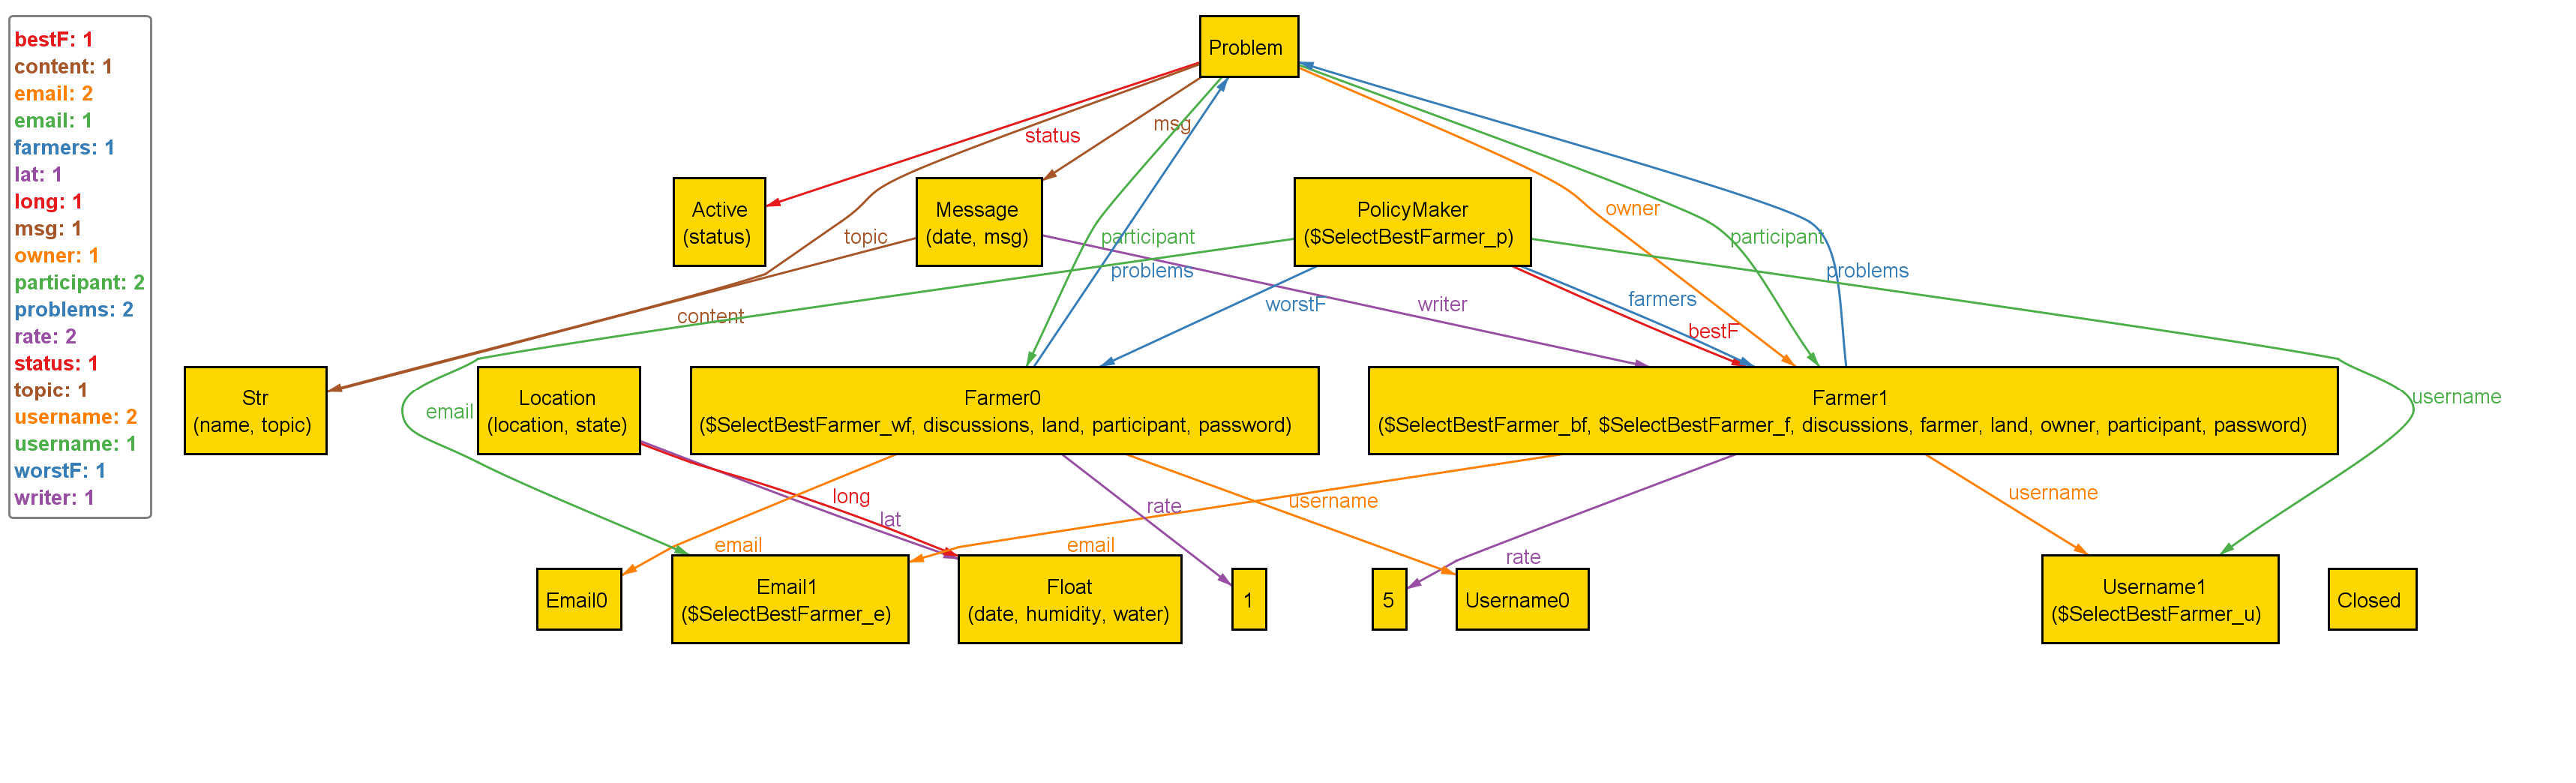
\includegraphics[width=0.9\textheight,keepaspectratio, angle=90]{figures/SelectBestandWorst.png}
  \caption{Select Best and Worst Farmers}
\end{figure}
\clearpage
%\subsection{Results of Assertions}
\subsection{Results of Predicates}
\begin{figure}[H]
  \centering
  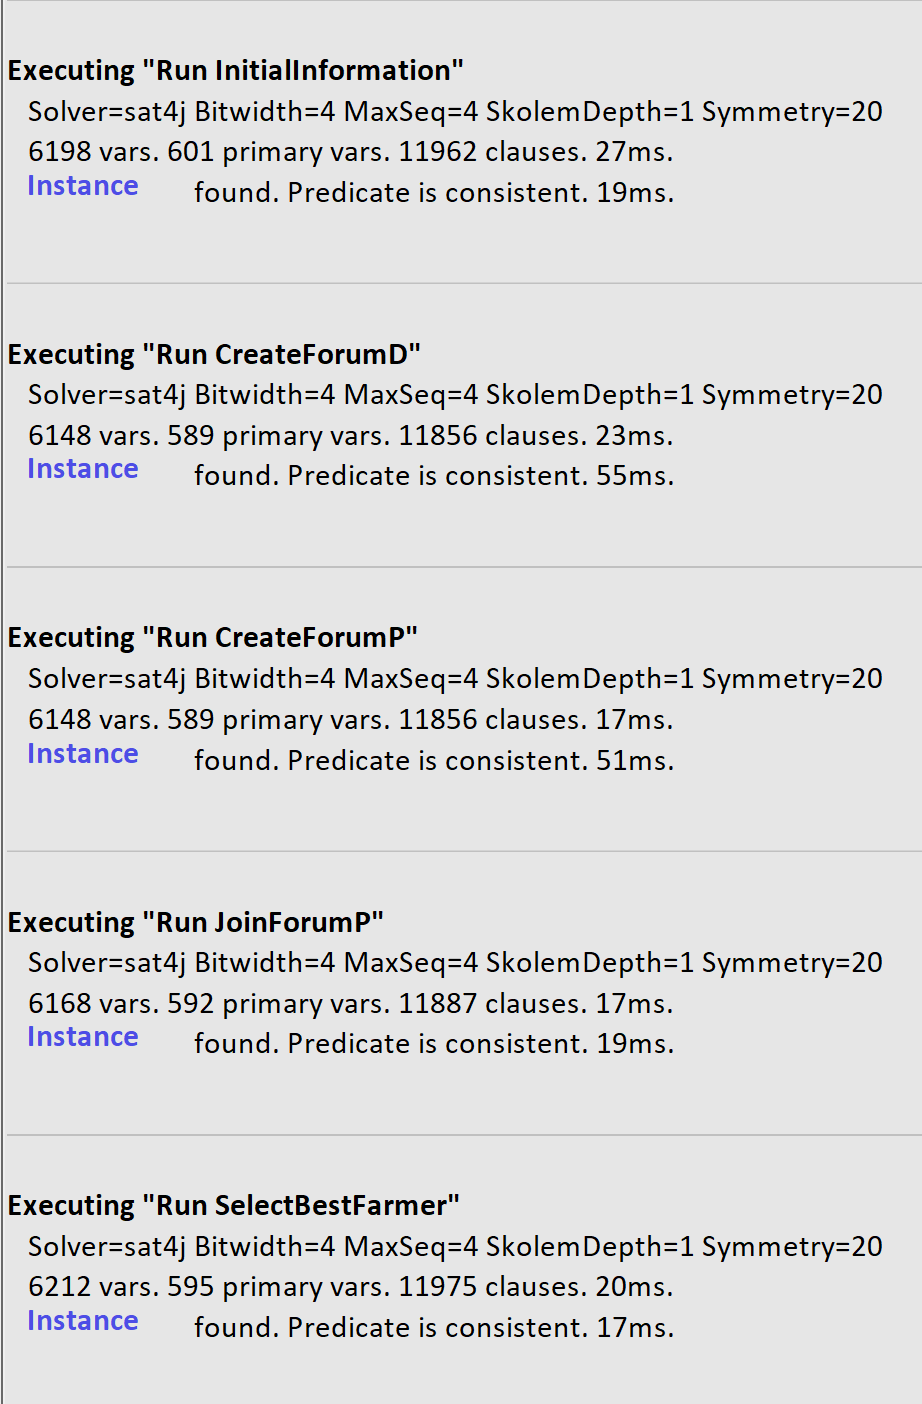
\includegraphics[width=0.6\textheight,keepaspectratio, angle=0]{figures/Executing.png}
  \caption{Executing Results}
\end{figure}
\clearpage
